% Introduction
\section{Introduction}
Recent advances in Large Language Models (LLMs) have introduced new possibilities for Automated Program Repair (APR). By understanding code context and iteratively testing their own fixes, LLMs can reduce the need for human intervention. This becomes more prominent in smaller projects, where the limited number of files and lines of code allows the entire context to fit within the model's input window.\\
However, this advantage diminishes as the size and complexity of a project grow. While larger codebases may technically fit within the context window, effective bug localization requires more than surface-level pattern recognition. It demands a deeper, semantic understanding of program behavior and structure something current LLMs are still not fully equipped to handle.\\
To address these limitations, we propose a pipeline that localizes bugs without relying on LLMs. By analyzing the codebase in tandem with the error trace, our method can more precisely identify the source of a bug. It comes within 3\% of the performance of Blaze (the current state-of-the-art). 
In our evaluation, this approach outperforms strategies that simply feed the full codebase to an LLM, offering a more scalable solution to the problem.

\begin{figure}[H]
\centering
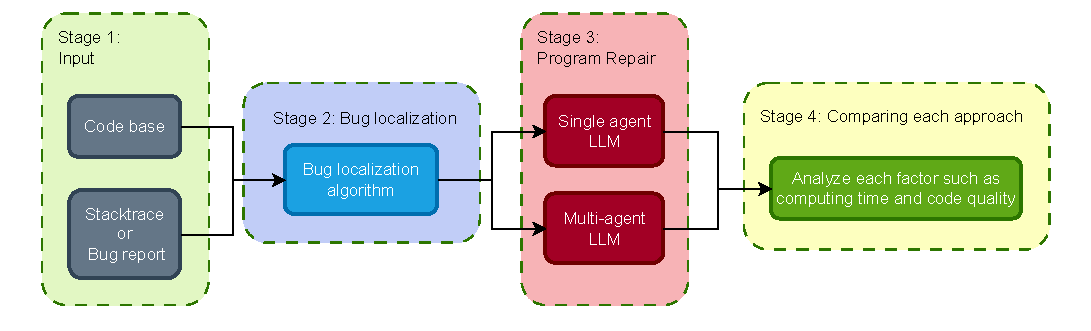
\includegraphics[width=1\columnwidth]{Figures/OverallView.pdf}
\caption{APR Pipeline}
\label{fig:apr_pipeline}
\end{figure}
